%!TEX root = ../main.tex 
\section{Experimental benchmarks}
\label{sec:rested-experiment}
We use the two benchmarks described in Subsection~\ref{subsec:rested-experiment1}.

\subsection{Simulated benchmark $\#$1 (2 arms).}
\begin{figure*}[ht]
\centering
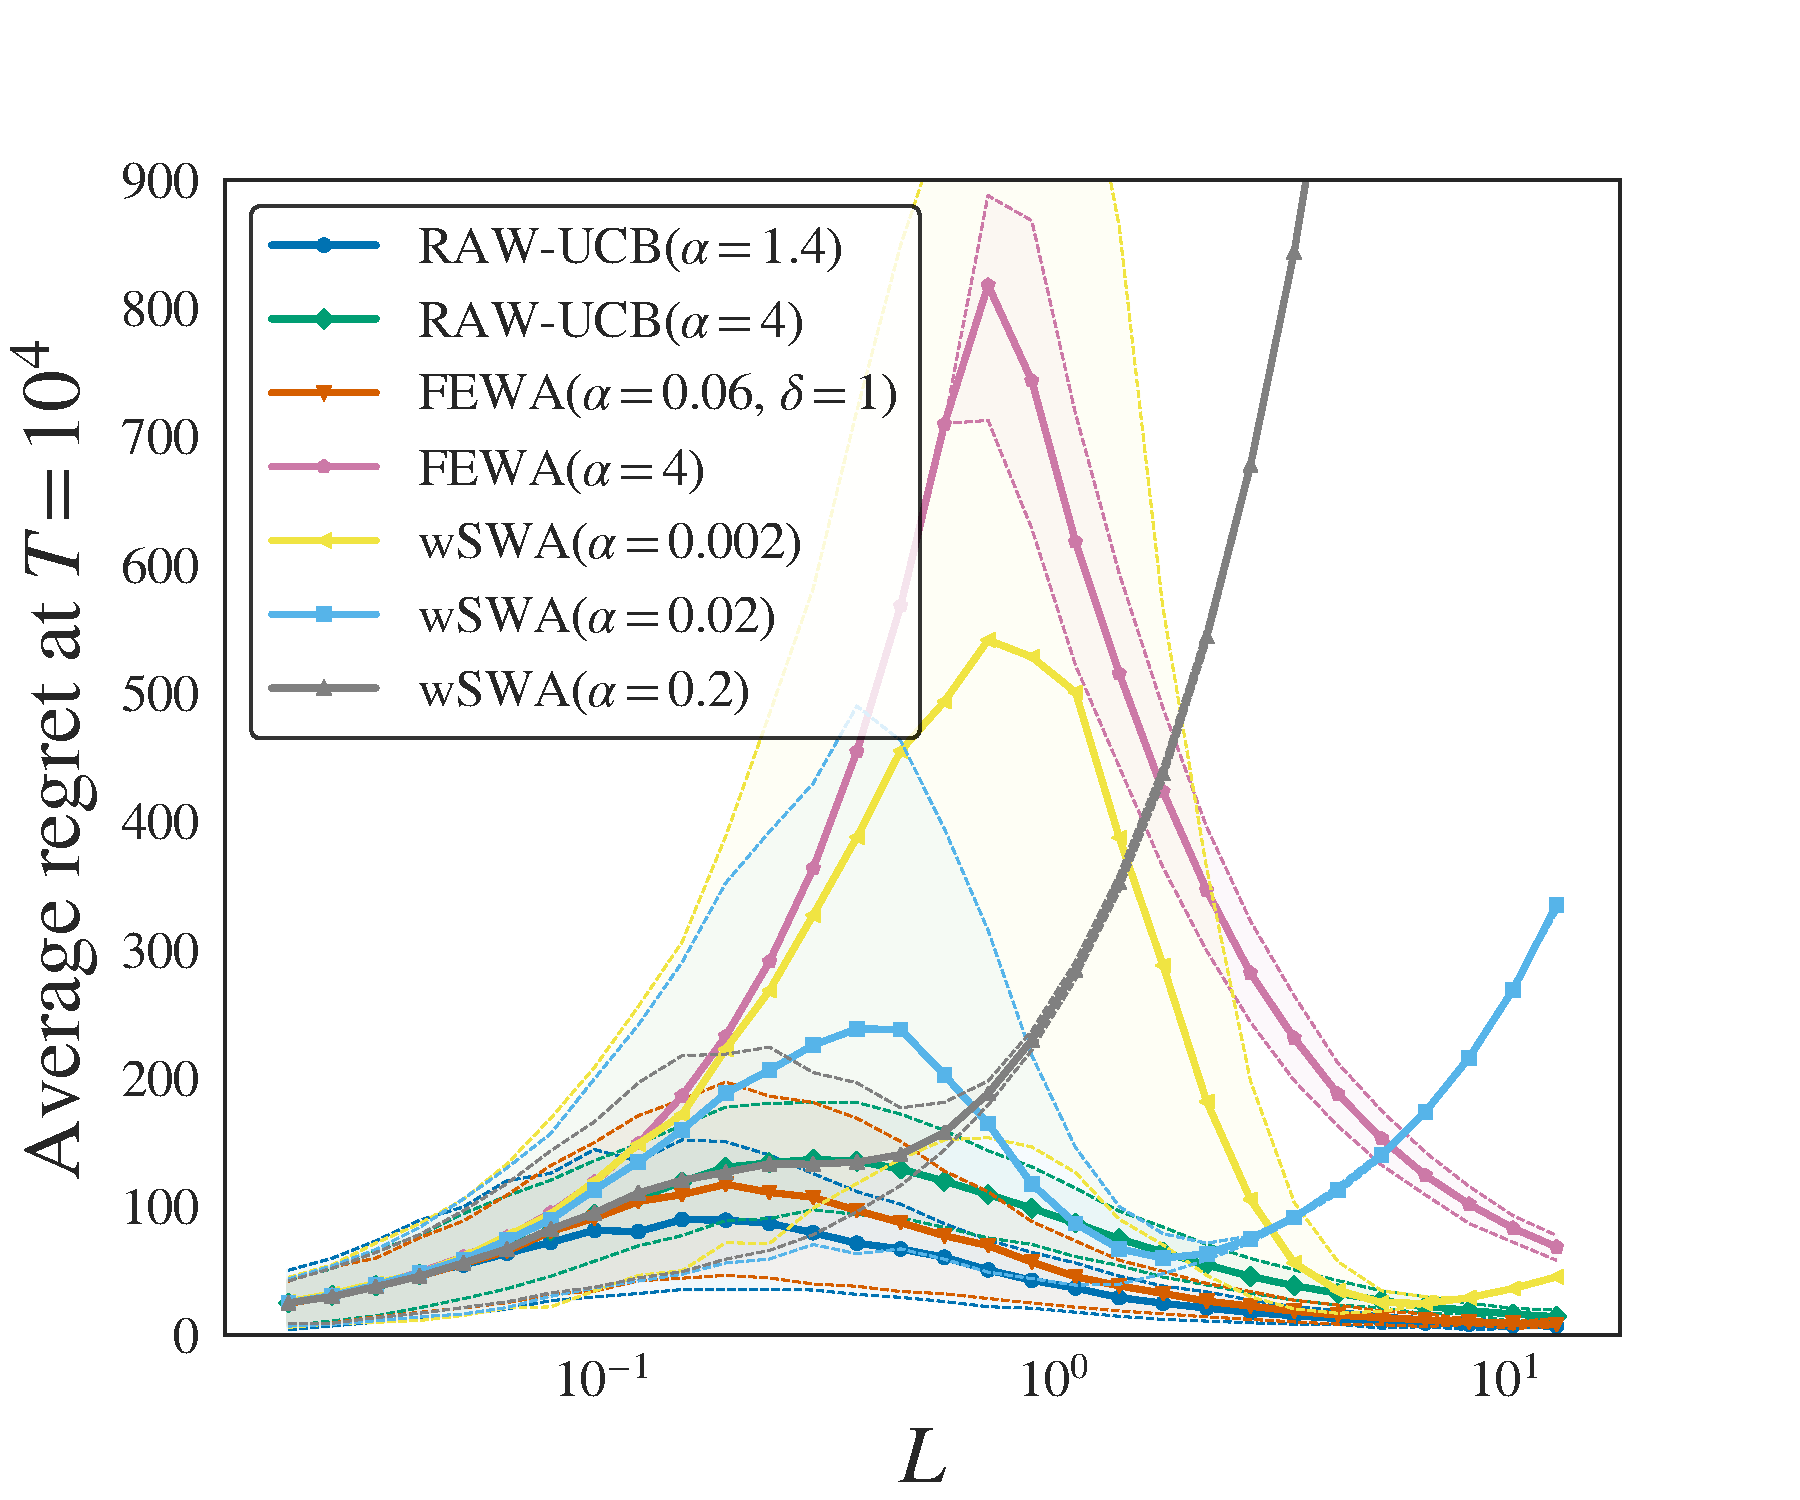
\includegraphics[clip, width= 0.51\textwidth]{2.1Rested/fig/fig1A_main.pdf}
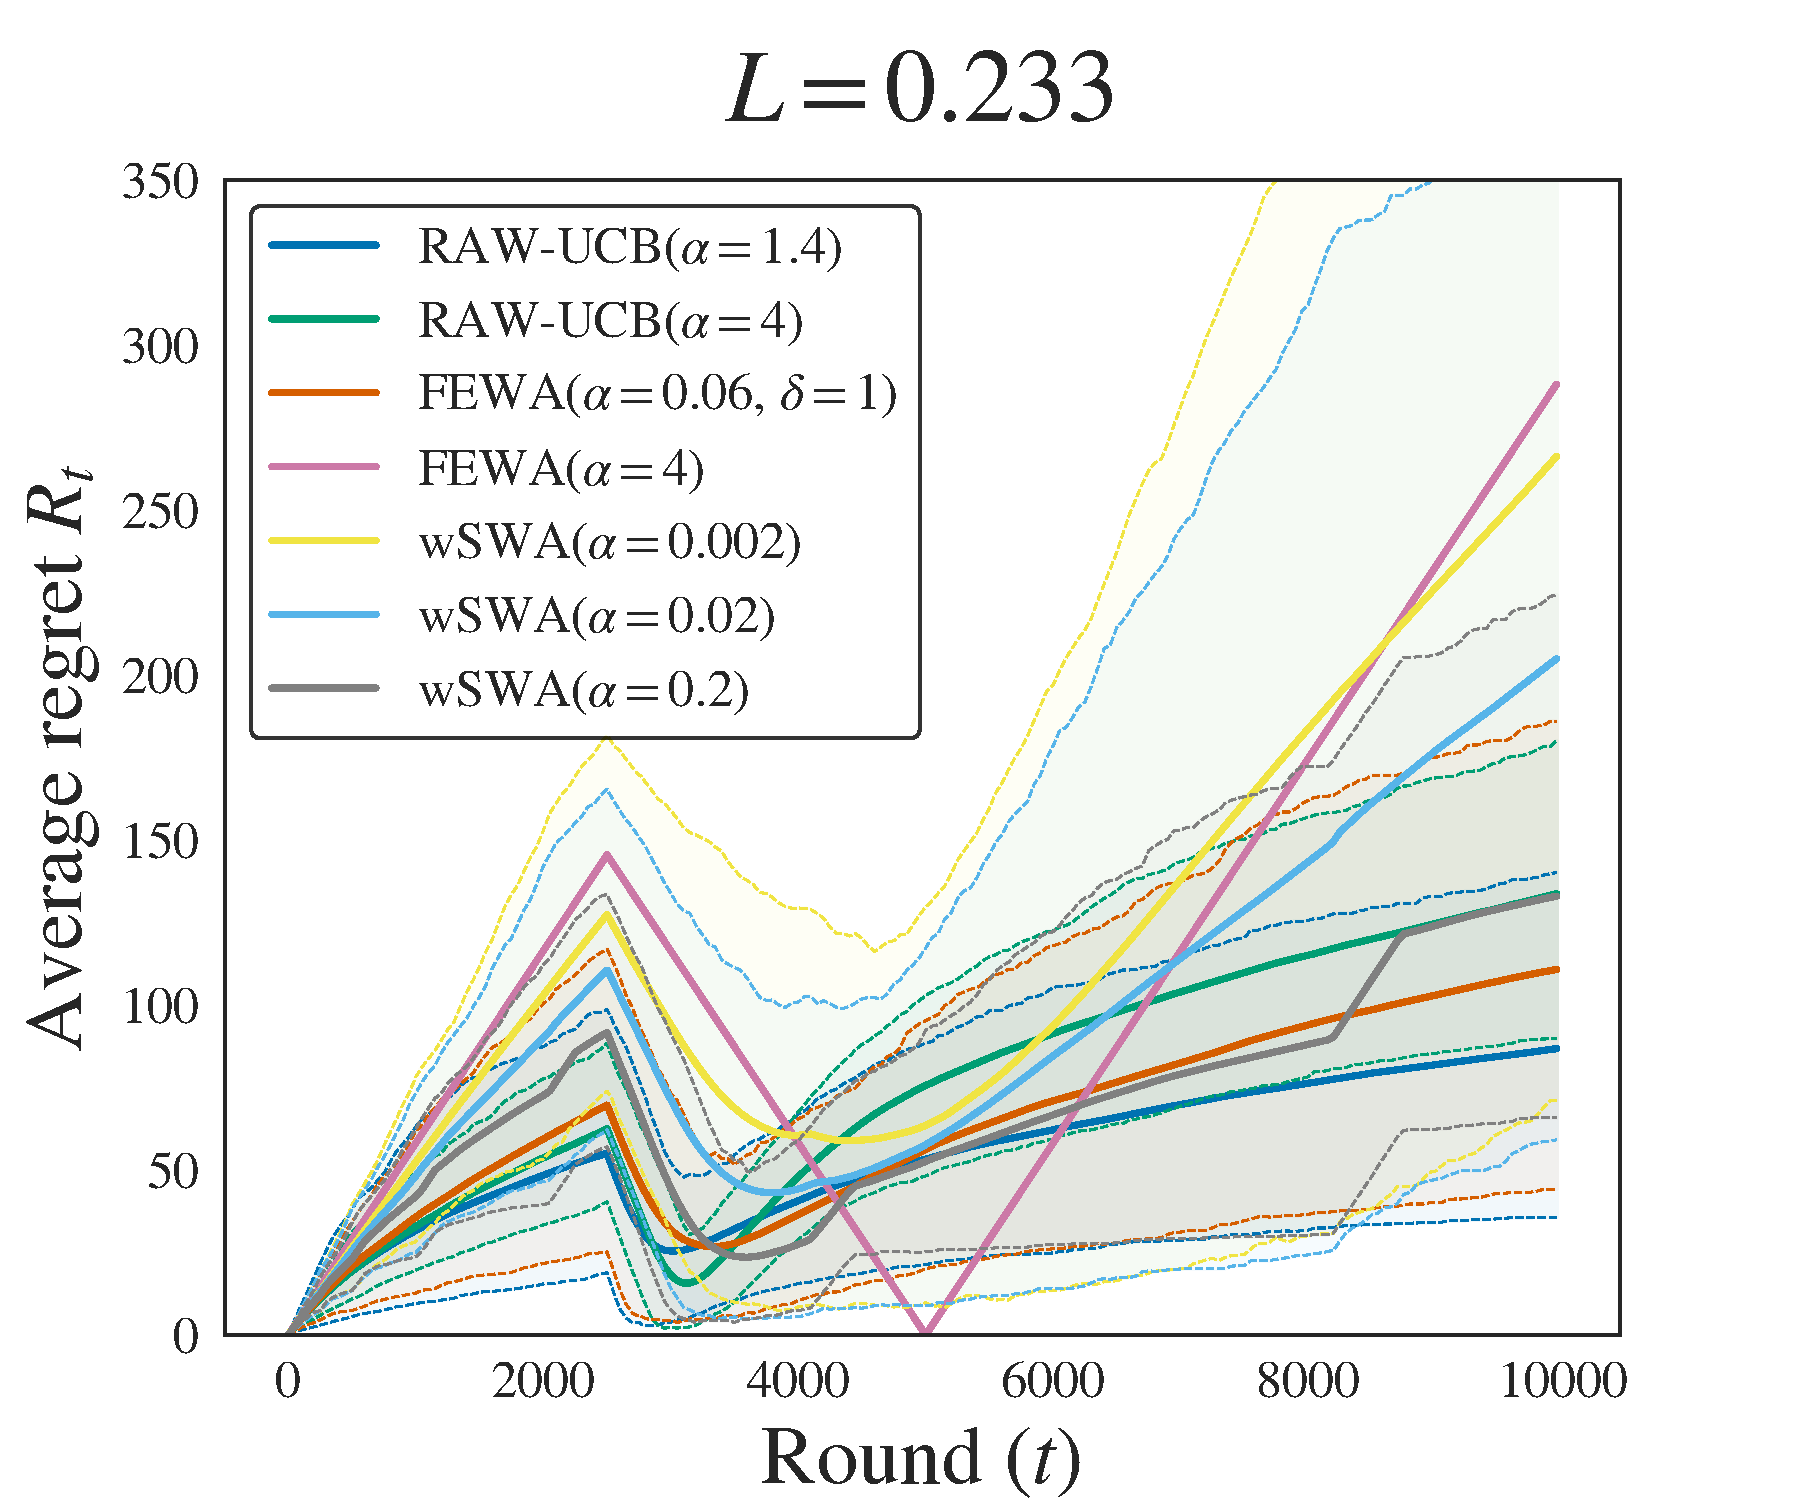
\includegraphics[clip, width= 0.49\textwidth]{2.1Rested/fig/fig1B_main.pdf}
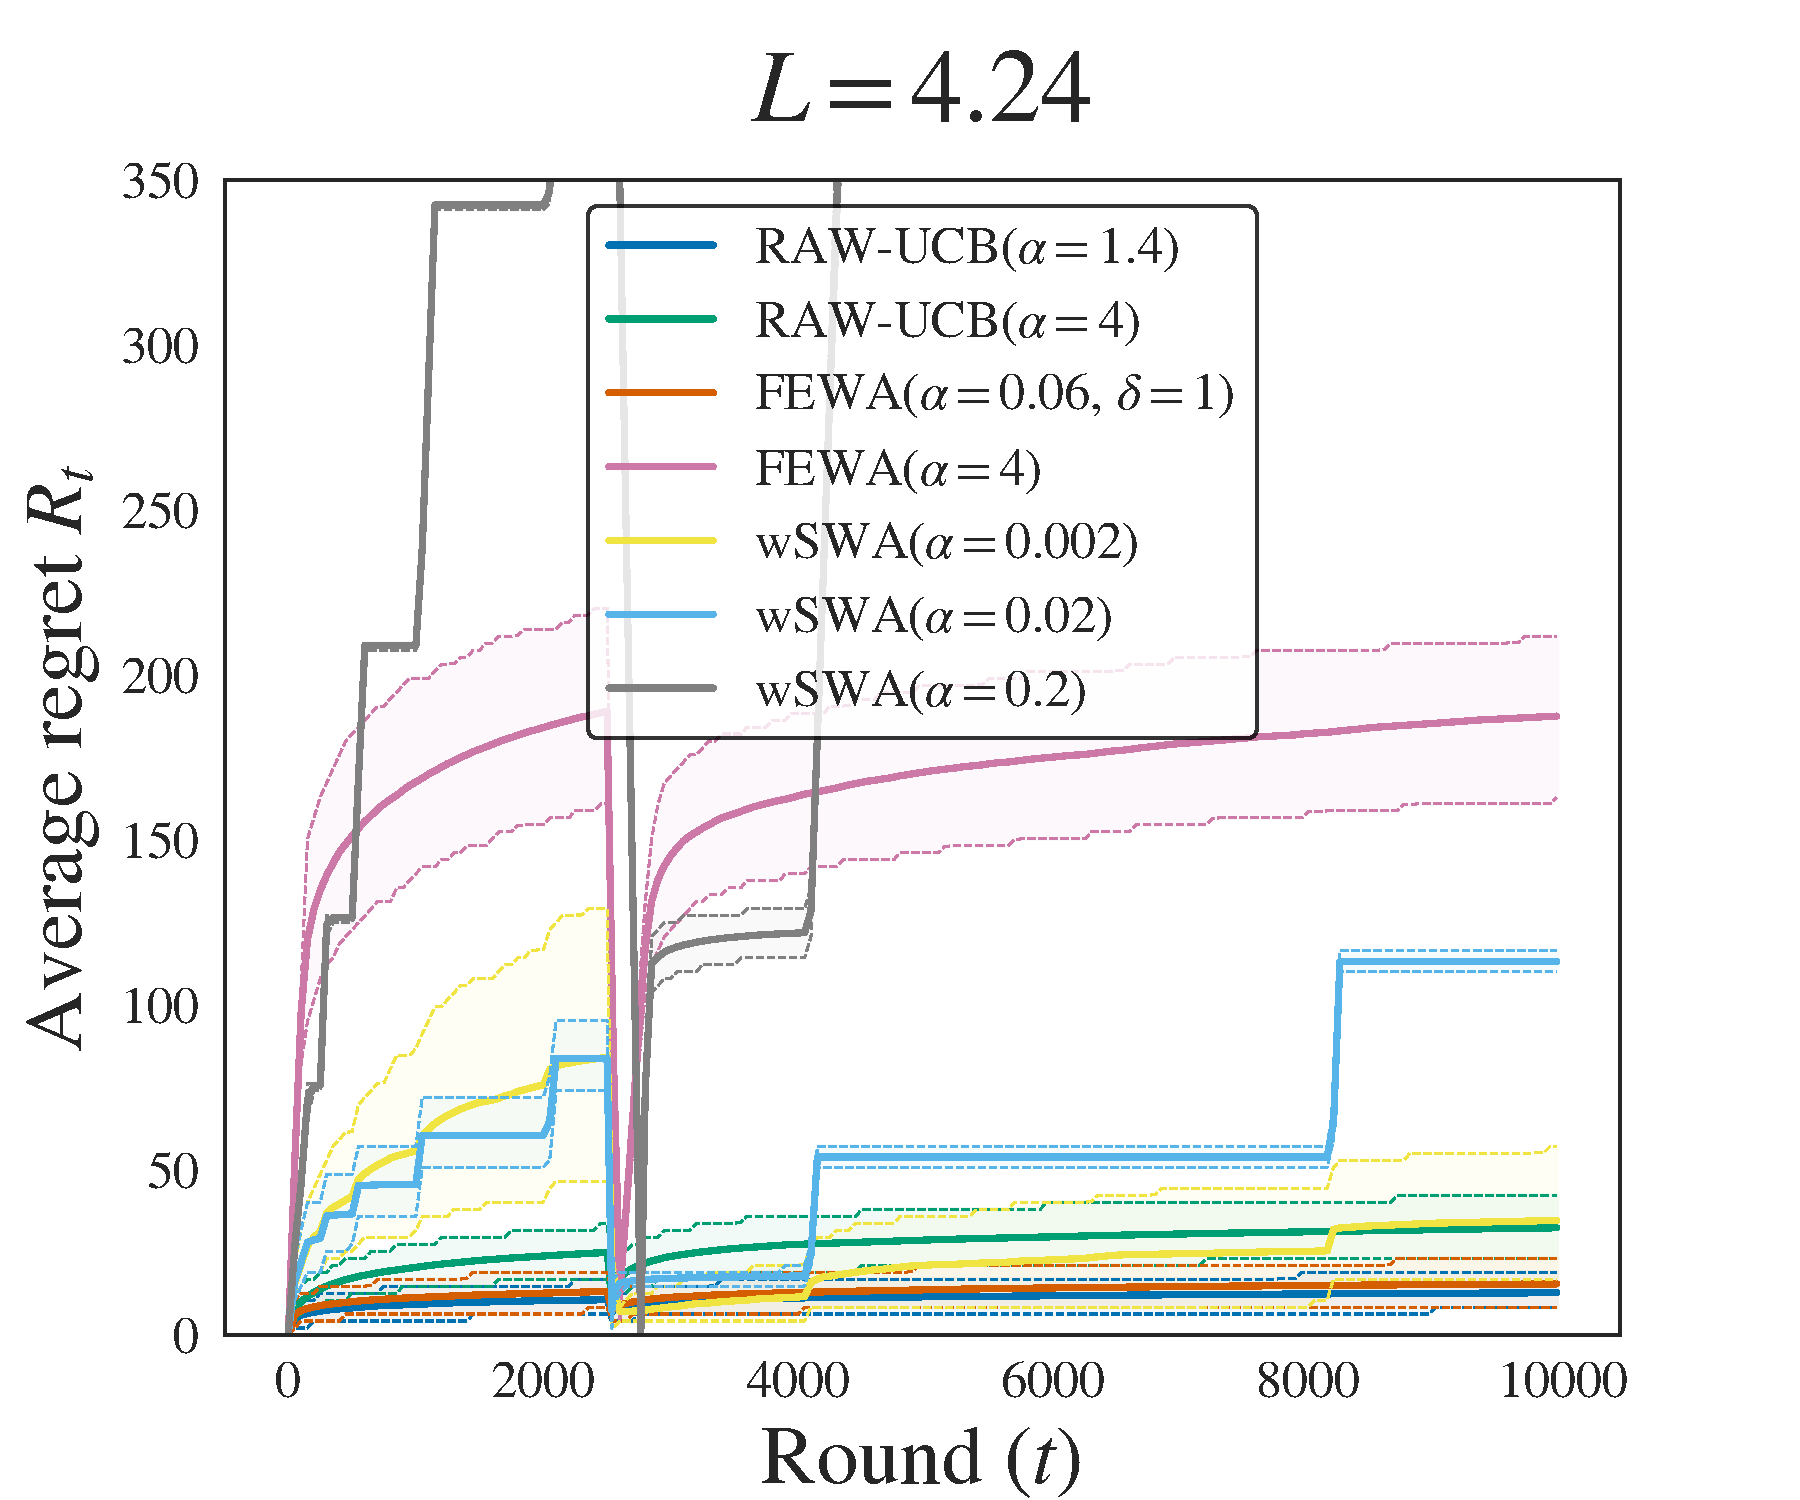
\includegraphics[clip, width= 0.49\textwidth]{2.1Rested/fig/fig1C_main.pdf}
\caption{\textbf{Top:} Regret at the end of the game for different values of $L$. \textbf{Bottom:} Regret across time for two values of $L$. Average over 1000 runs. We highlight the $\left[10\%, 90\%\right]$ confidence region.}
\label{fig:rested-exp1}
\end{figure*}

\paragraph{Algorithms.} We display the performance of \RAWUCB and \FEWA for two versions of each algorithm: with the theoretical tuning $\alpha = 4$; and with the empirical tuning $\alpha_{\mathrm{R}} = 1.4$ and $\alpha_{\mathrm{F}} = 0.06$. These two values are selected by grid-search. Though there are 30 different problems (for different $L$), the best tuning of $\alpha$ is the same for all the considered problem. We also include the three versions of \wSWA that we displayed in Subsection~\ref{subsec:rested-experiment1}.


\paragraph{Results - {\RAWUCB} versus {\FEWA}.} We compare \RAWUCB and \FEWA both for theoretical and empirical tuning. For theoretical tuning, we see in Figure~\ref{fig:rested-exp1} (top), that \RAWUCB outperforms \FEWA on all sizes of decays by a factor $\sim 4$ which is predicted by our theory. Indeed, there is also a factor 4 between the two problem-dependent upper-bounds (Theorem~\ref{th:rested-PD}). 

Surprisingly, for empirical tuning, the average performances of the two algorithms are much closer. We also notice that there is a larger variance in \FEWA's result compared to \RAWUCB. This is not surprising because we had to drastically reduce the confidence bounds to make \FEWA practical. It means that empirical \FEWA filters arms based only on a handful of samples. This bet leads to both very good and very bad runs. Last, Figure~\ref{fig:rested-exp1} (bottom) shows that \RAWUCB outperforms \FEWA at almost any time $t$, both on easy ($L=4.24$) and difficult ($L=0.233$) problems. The only round at which \FEWA shows better performance than \RAWUCB is after the regret decay. It is because \FEWA was less good at identifying the best arm in the first part of the game. Hence, just after the decay, it pulls more the other arm - which has become optimal. 

In the following, we will compare \RAWUCB with \wSWA. Notice that a similar comparison can hold for \FEWA ($\alpha=0.06$).

\paragraph{Results - Problem dependent performance and the impact of L.} \RAWUCB with the best empirical tuning improves over \wSWA on each problem (Figure~\ref{fig:rested-exp1} (top)). \RAWUCB with the theoretical tuning recovers quite good performance as well. 

In this setting, $L$ has two different meanings. It is the maximum decay per round (noted as $L$ in the theoretical section) and the gap between arms $\Delta_{2,h} = \nicefrac{L}{2}$ (for any $h$). According to our problem-dependent bound in Theorem~\ref{th:rested-PD}, the regret bound converges to $\cO\pa{KL}$ when $L$ and $\Delta_{2,h}$ are large with respect to $\sigma$. It tends to show that setup where arms are well separated from each other are easy problems for \FEWA and \RAWUCB. It is indeed confirmed in Figure~\ref{fig:rested-exp1} (top), where the regret of \FEWA and \RAWUCB converges to $\nicefrac{L}{2}$ when $L$ is large.

\paragraph{Results - Worst-case improvement.}
In Figure~\ref{fig:rested-exp1} (top), the worst regret for any of the two versions of \RAWUCB is smaller than the worst regret of any of the three versions \wSWA. Moreover, we remark that the regret at the round $T$ has one maximum for the variation of $L$ for \RAWUCB. This is not the case for \wSWA where the regret increases again for large values of $L$.

It confirms our analysis. Indeed, Theorem~\ref{th:rested-PI} shows a larger regret rate than Proposition~\ref{prop:SWA}. Moreover, the analysis shows that the worst cases for \RAWUCB correspond to cases where the learner does $\cO\pa{T}$ mistakes of intermediate size  $\cO\pa{\sqrt{\nicefrac{K}{T}}}$ which corresponds to the single maximum in Figure~\ref{fig:rested-exp1} (top).  

\paragraph{Results - Tuning and agnostic algorithms.}
Figure~\ref{fig:rested-exp1} (top) confirms that \FEWA and \RAWUCB do not rely on the knowledge of $L$. Indeed, the optimal tuning is the same for all the 30 problems. By contrast, the performance of \wSWA depends critically on the prior knowledge of  $L$: each of the three displayed tunings is the best for a specific range of $L$. 

Figure~\ref{fig:rested-exp1} (bottom) shows the advantage of anytime algorithms compared to the doubling trick. Indeed, the periodic restarts are quite expensive for \wSWA.  

\paragraph{Results - High-probability.}
We see that the variance of \wSWA is quite large for intermediate values of $L$. It confirms the analysis of \wSWA which shows two sources of the regret: the variance and the bias of the index. The regrets caused by variance has itself a large variance. Indeed, the sub-optimal arms are often correctly estimated, and hence not pulled by the index policy. It leads to many good runs of \wSWA. However, there are still many runs on which there is a sufficient deviation in the indexes which leads to very large regret. 

By contrast, the variance in the results is much more controlled by \RAWUCB and \FEWA. Indeed, when the statistics of these algorithms are not significant enough they tend to explore which leads to less large deviation of the regret. 

\subsection{Simulated benchmark $\#$2 (10 arms).}

\begin{figure*}[t]
\centering
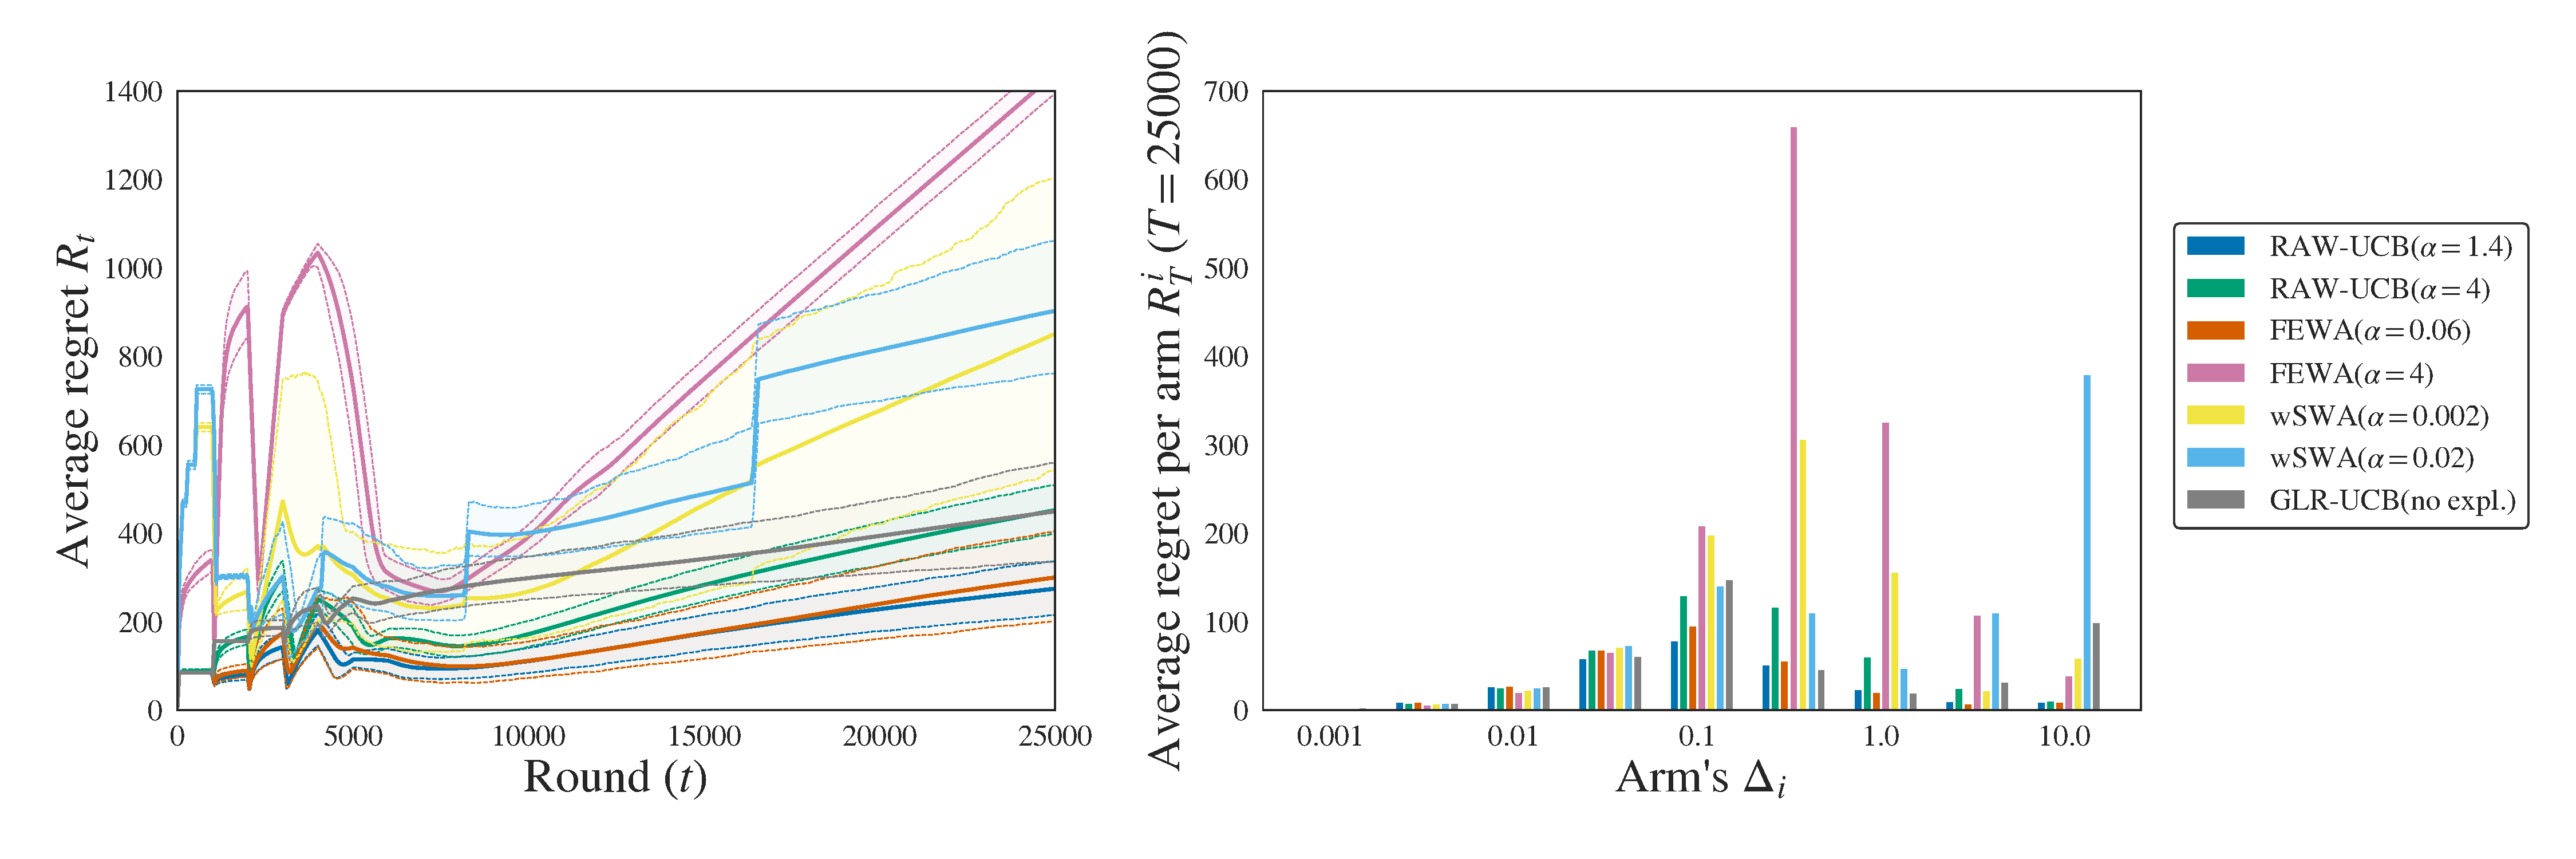
\includegraphics[width = 0.99 \textwidth]{2.1Rested/fig/fig2_main.pdf}
\caption{\textbf{Left:} Regret at the end of the game for different values of $L$. \textbf{Middle, Right:} Regret across time for two values of $L$. Average over 1000 runs. We highlight the $\left[10\%, 90\%\right]$ confidence region.}
\label{fig:rested-exp2}
\end{figure*}

\paragraph{Algorithms.} We display the same two versions of \FEWA and \RAWUCB. We also show the three best algorithms presented in Subsection~\ref{subsec:rested-experiment1}: two versions of \wSWA with $\alpha\in \left\{0.002, 0.02\right\}$ and \GLRUCB with no exploration. 

\paragraph{Results.}
The comparison between \RAWUCB, \FEWA, and \wSWA leads to a similar conclusion than for the two-arm bandit experiment. \RAWUCB and \FEWA show superior performance, except for the theoretical tuning of \FEWA which is too conservative. 

In particular, these algorithms show a better adaptation to each arm's gap. Indeed, the regret per arm is more controlled, especially for large values of the gaps, on which \wSWA suffers a large regret. There is also less deviation in the regret and we see the benefits of avoiding the doubling trick. 

In the two-arm setup with a single decay, it is possible to find a value of $\alpha$ for which \wSWA is correctly tuned for the specific decay. For instance, for $L\in \left[ 1, 3\right]$, \wSWA with $\alpha = 0.02 $ has almost the same performance than \RAWUCB (Fig.~\ref{fig:rested-exp1}). In the ten-arm setup with multiple decays, this is not possible anymore. Indeed, since there are several dropping values for each arm, there exists at least one arm on which the fixed window of \wSWA is not correctly tuned. For instance, for $\alpha = 0.002$ , \wSWA suffers a large regret on the arm with $\Delta_i = 0.3$. For \wSWA with $\alpha = 0.02$, the regret is large when $\Delta_i = 10$.

\RAWUCB and \FEWA also improve over \GLRUCB when their confidence bounds are tuned. We recall that \GLRUCB is an algorithm that uses a classical UCB index with a change detection procedure. When the change-detection procedure triggers, it erases the history of the changing arm. Notice that the confidence bounds of the index of \GLRUCB are already well-tuned, as they use the same confidence bounds as the asymptotic optimal tuning of \UCB. \GLRUCB shows sub-optimal performance on two arms $\Delta_i \in \left\{0.1, 10\right\}$. \GLRUCB suffers from the late restart for $\Delta_i = 0.1$.  Indeed, the change-point is hard to detect, and the index of the sub-optimal value is positively biased while it has not restarted. For $\Delta_i = 10$, the large regret of \GLRUCB is due to an implementation artefact. Indeed, we used the fast implementation for the change detector (by default in \citep{SMPyBandits}). It speeds up the algorithm but it can delay the change-detection scheme (by 10 pulls in this case). This delay leads to large regret when the mistake associated with each arm is large (as it is the case for $\Delta_i=10$).

\paragraph{Running time.}
\begin{table}[H]
\centering
\begin{tabular}{|c|c|}
\hline
\textbf{Policy} &\textbf{Running time (s)} \\ \hline
\FEWA($\alpha = 0.06$)    & 91                      \\ 
\FEWA($\alpha = 4$)      & 780                     \\ \hline
\RAWUCB ($\alpha = 1.4$) & 27                      \\
\RAWUCB($\alpha = 4$)    & 25                      \\ \hline
\wSWA($\alpha = 0.002$)   & 1                       \\ 
\wSWA($\alpha = 0.02$)    & 1                       \\ \hline
\GLRUCB          & 46 \\ \hline
\end{tabular}
  \caption{Average running time for the 10-arms experiment in seconds.}
  \label{tab:time-fig2}
\end{table}

In Table~\ref{tab:time-fig2}, we display the running time for this experiment. The computational experiments were conducted using the Grid’5000 experimental testbed \citep{grid5000}. For meaningful comparison, all the algorithms run on the same "Grenoble/dahu" cluster (2 CPUs Intel Xeon Gold 6130, 16 cores/CPU, 192GB RAM, 223GB SSD, 447GB SSD, 3726GB HDD, 1 x 10Gb Ethernet, 1 x 100Gb Omni-Path). 

\RAWUCB runs 25 times slower than \wSWA. We will provide a computational analysis in the next section but we can already relate this increased running time with the higher number of statistics \RAWUCB update and compare at each round.

The $\alpha$ parameter of \FEWA has a large impact on the running time. Indeed, the larger the $\alpha$, the less aggressive are the filters, the longer it takes to reach the end of the filtering process. Yet, even when $\alpha$ is small, \FEWA is slower than \RAWUCB. This is a consequence of the simplicity of the index policy over the filtering procedure. Indeed, in Python, we can use the fast C++ implementation of the scientific computing library Numpy to perform the most classical operations. Hence, for \RAWUCB, we only use the NumPy functions $\argmax$ and $\min$ to choose the next arm. For \FEWA, the comparison part is more custom: we had to implement the while-loop at Line~\ref{algline:fewa-while} with a Python loop, which is known to be quite slow. Notice that since the two algorithms use the same statistics we use the same function \UPDATE in both algorithms.

\GLRUCB is slower than \RAWUCB. Notice that it is already a fast version of \GLRUCB which runs the change-detection subroutine sparsely (approximately 10 to 100 times faster than the original \GLRUCB).
\begin{remark}
We emphasize the better characteristics of \RAWUCB over \FEWA: better bounds, better empirical performances, easier and faster implementation, a better agreement between theory and practice, closer to the classical \UCB. For these reasons, we will focus our future empirical investigation on \RAWUCB.
\end{remark}